\documentclass[
version=last,toc=bib,toc=graduated,toc=index,toc=listof,9pt,openany]{scrbook}
%\pdfminorversion=4
\usepackage{polyglossia}
\setdefaultlanguage{english}

\setmainfont{Source Sans Pro}
\setsansfont{Source Sans Pro}

\usepackage{ifmtarg}
\usepackage{ifthen}
\usepackage{etoolbox} % \ifstrempty

\usepackage{geometry}
\geometry{%a6paper
paperwidth=125mm, paperheight=168mm, 
portrait,
top=22mm,
inner=22mm,
outer=20mm,
bottom=25mm,
headsep=3mm,
footskip=12mm
}

\usepackage{ragged2e} % nicer typesetting (hyphenation) for non raggedright and raggedleft
\usepackage{lscape}
\setlength{\parskip}{0pt}

\usepackage{relsize}

\clubpenalty=10000
\widowpenalty=10000 
\displaywidowpenalty=10000

\usepackage[]{microtype}

\usepackage{graphicx} % graphics

% search path for images
\graphicspath{{images-print/}{icons/}{extra-pages/}{wallpaper/}}
\usepackage{wrapfig}  % sponsor logos wrapped with text

\usepackage{tabu}
\usepackage{tabularx}
\usepackage{longtable}
\usepackage[table,cymk]{xcolor}
\usepackage{colortbl}

% embed PDF pages
% pdfpages must not be loaded before colortbl!
\usepackage{pdfpages}
% TikZ must not be loaded before colortbl
\usepackage{tikz}

\usepackage{multirow}
\usepackage{booktabs}
\usepackage{array}

% multiple text columns (list of thanks)
\usepackage{multicol}

\usepackage{refcount} % calculation of the page where the map is located

% page background
\usepackage[manualmark]{scrlayer-scrpage}
\pagestyle{scrplain}

\newcommand{\acro}[1]{{\textsmaller{#1}}} % macro for abbreviations with more than one capitalised letter


% title/metadata
\title{State of the Map 2018}
\subtitle{Programme}
\author{OpenStreetMap Foundation}
\date{\today}

\clearscrheadings

% page numbers
\cfoot[\begin{small}\pagemark\end{small}]{\begin{small}\pagemark\end{small}}
\ofoot[]{}
\ifoot[]{}
\pagestyle{scrplain}

\linespread{1.15}

% include our custom macros
\input{abstract-commands}
% OSMF
\DeclareNewLayer[background,%
  width=125mm,%
  height=168mm,%
  contents={%
    \includegraphics{wallpaper/osmf.pdf}%
  }%
]{osmfmap}
\newpairofpagestyles{osmf}{}
\AddLayersAtBeginOfPageStyle{osmf}{osmfmap}

% metro map of Milan
\DeclareNewLayer[background,%
  width=125mm,%
  height=168mm,%
  contents={%
    \includegraphics{wallpaper/metro.pdf}%
  }%
]{metromap}
\newpairofpagestyles[scrheadings]{metro}{}
\AddLayersAtBeginOfPageStyle{metro}{metromap}

% Microsoft advertisement
\DeclareNewLayer[background,%
  width=125mm,%
  height=168mm,%
  hoffset=-0.4mm,%
  contents={%
    \includegraphics{sponsors/microsoft-cropped-compressed.pdf}%
  }%
]{microsoftadvertisement}
\newpairofpagestyles{sponsor-microsoft}{}
\AddLayersAtBeginOfPageStyle{sponsor-microsoft}{microsoftadvertisement}

% Facebook advertisement
\DeclareNewLayer[background,%
  width=125mm,%
  height=168mm,%
  contents={%
    \includegraphics{sponsors/facebook.pdf}%
  }%
]{facebookadvertisement}
\newpairofpagestyles{sponsor-facebook}{}
\AddLayersAtBeginOfPageStyle{sponsor-facebook}{facebookadvertisement}

% Mapbox advertisement
\DeclareNewLayer[background,%
  width=125mm,%
  height=168mm,%
  contents={%
    \includegraphics{sponsors/mapbox.pdf}%
  }%
]{mapboxadvertisement}
\newpairofpagestyles{sponsor-mapbox}{}
\AddLayersAtBeginOfPageStyle{sponsor-mapbox}{mapboxadvertisement}

% Kaart/Maps.Me advertisement
\definecolor{kaartblack}{cmyk}{0.16 0.11 0.0 0.78}
%\definecolor{mapsmegrey}{cmyk}{0.0 0.0 0.0 0.20}
\definecolor{mapsmegrey}{HTML}{F4F4F4}
\DeclareNewLayer[background,%
  width=125mm,%
  height=168mm,%
  hoffset=5mm,
  voffset=5mm,
  contents={%
    \begin{tikzpicture}[x=1mm, y=1mm]
      \fill [kaartblack] (0,0) rectangle (115,79);
      \fill [mapsmegrey] (0,79) rectangle (115,158);
    \end{tikzpicture}
  }%
]{kaartblackbackground}
\DeclareNewLayer[background,%
  width=68.843mm,%
  height=15.495mm,%
  hoffset=28.08mm,
  voffset=105.505mm,
  contents={%
    \input{images-print/kaart.tex}
  }%
]{kaarttext}
\DeclareNewLayer[background,%
  width=105mm,%
  height=74mm,%
  hoffset=10mm,
  voffset=10mm,
  contents={%
    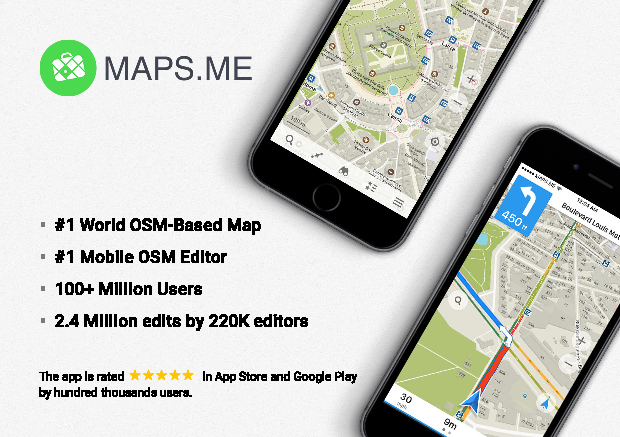
\includegraphics[width=105mm]{images-print/mapsme-compressed.pdf}
  }%
]{mapsmelogo}
\newpairofpagestyles{sponsor-kaartmapsme}{}
\AddLayersAtBeginOfPageStyle{sponsor-kaartmapsme}{kaarttext}
\AddLayersAtBeginOfPageStyle{sponsor-kaartmapsme}{mapsmelogo}
\AddLayersAtBeginOfPageStyle{sponsor-kaartmapsme}{kaartblackbackground}
\AddLayersAtBeginOfPageStyle{sponsor-kaartmapsme}{cropmarksevery}

% Immobilare advertisement
\DeclareNewLayer[background,%
  width=125mm,%
  height=168mm,%
  contents={%
    \includegraphics{sponsors/immobiliare.pdf}%
  }%
]{immobiliareadvertisement}
\newpairofpagestyles{sponsor-immobiliare}{}
\AddLayersAtBeginOfPageStyle{sponsor-immobiliare}{immobiliareadvertisement}

% Telenav advertisement
\DeclareNewLayer[background,%
  width=125mm,%
  height=168mm,%
  contents={%
    \includegraphics{sponsors/telenav-blue-bottom.pdf}%
  }%
]{telenavblue}
\DeclareNewLayer[background,%
  width=105mm,%
  height=148mm,%
  hoffset=10mm,%
  voffset=10mm,%
  contents={%
    \includegraphics{sponsors/telenav.pdf}%
  }%
]{telenav}
\newpairofpagestyles{sponsor-telenav}{}
\AddLayersAtBeginOfPageStyle{sponsor-telenav}{telenav}
\AddLayersAtBeginOfPageStyle{sponsor-telenav}{telenavblue}

% Garmin and Mapillary advertisement
\DeclareNewLayer[background,%
  width=115mm,%
  height=79mm,%
  hoffset=5mm,
  voffset=84mm,
  contents={%
    \includegraphics{sponsors/garmin-compressed.pdf}%
  }%
]{garmin}
\DeclareNewLayer[background,%
  width=115mm,%
  height=79mm,%
  hoffset=5mm,%
  voffset=5mm,%
  contents={%
    \includegraphics{sponsors/mapillary-compressed.pdf}%
  }%
]{mapillary}
\newpairofpagestyles{sponsor-garmin-mapillary}{}
\AddLayersAtBeginOfPageStyle{sponsor-garmin-mapillary}{garmin}
\AddLayersAtBeginOfPageStyle{sponsor-garmin-mapillary}{mapillary}
\AddLayersAtBeginOfPageStyle{sponsor-garmin-mapillary}{cropmarksevery}

% double map page
\DeclareNewLayer[background,%
  evenpage,
  width=115mm,%
  height=158mm,%
  hoffset=5mm,
  voffset=5mm,
  contents={%
    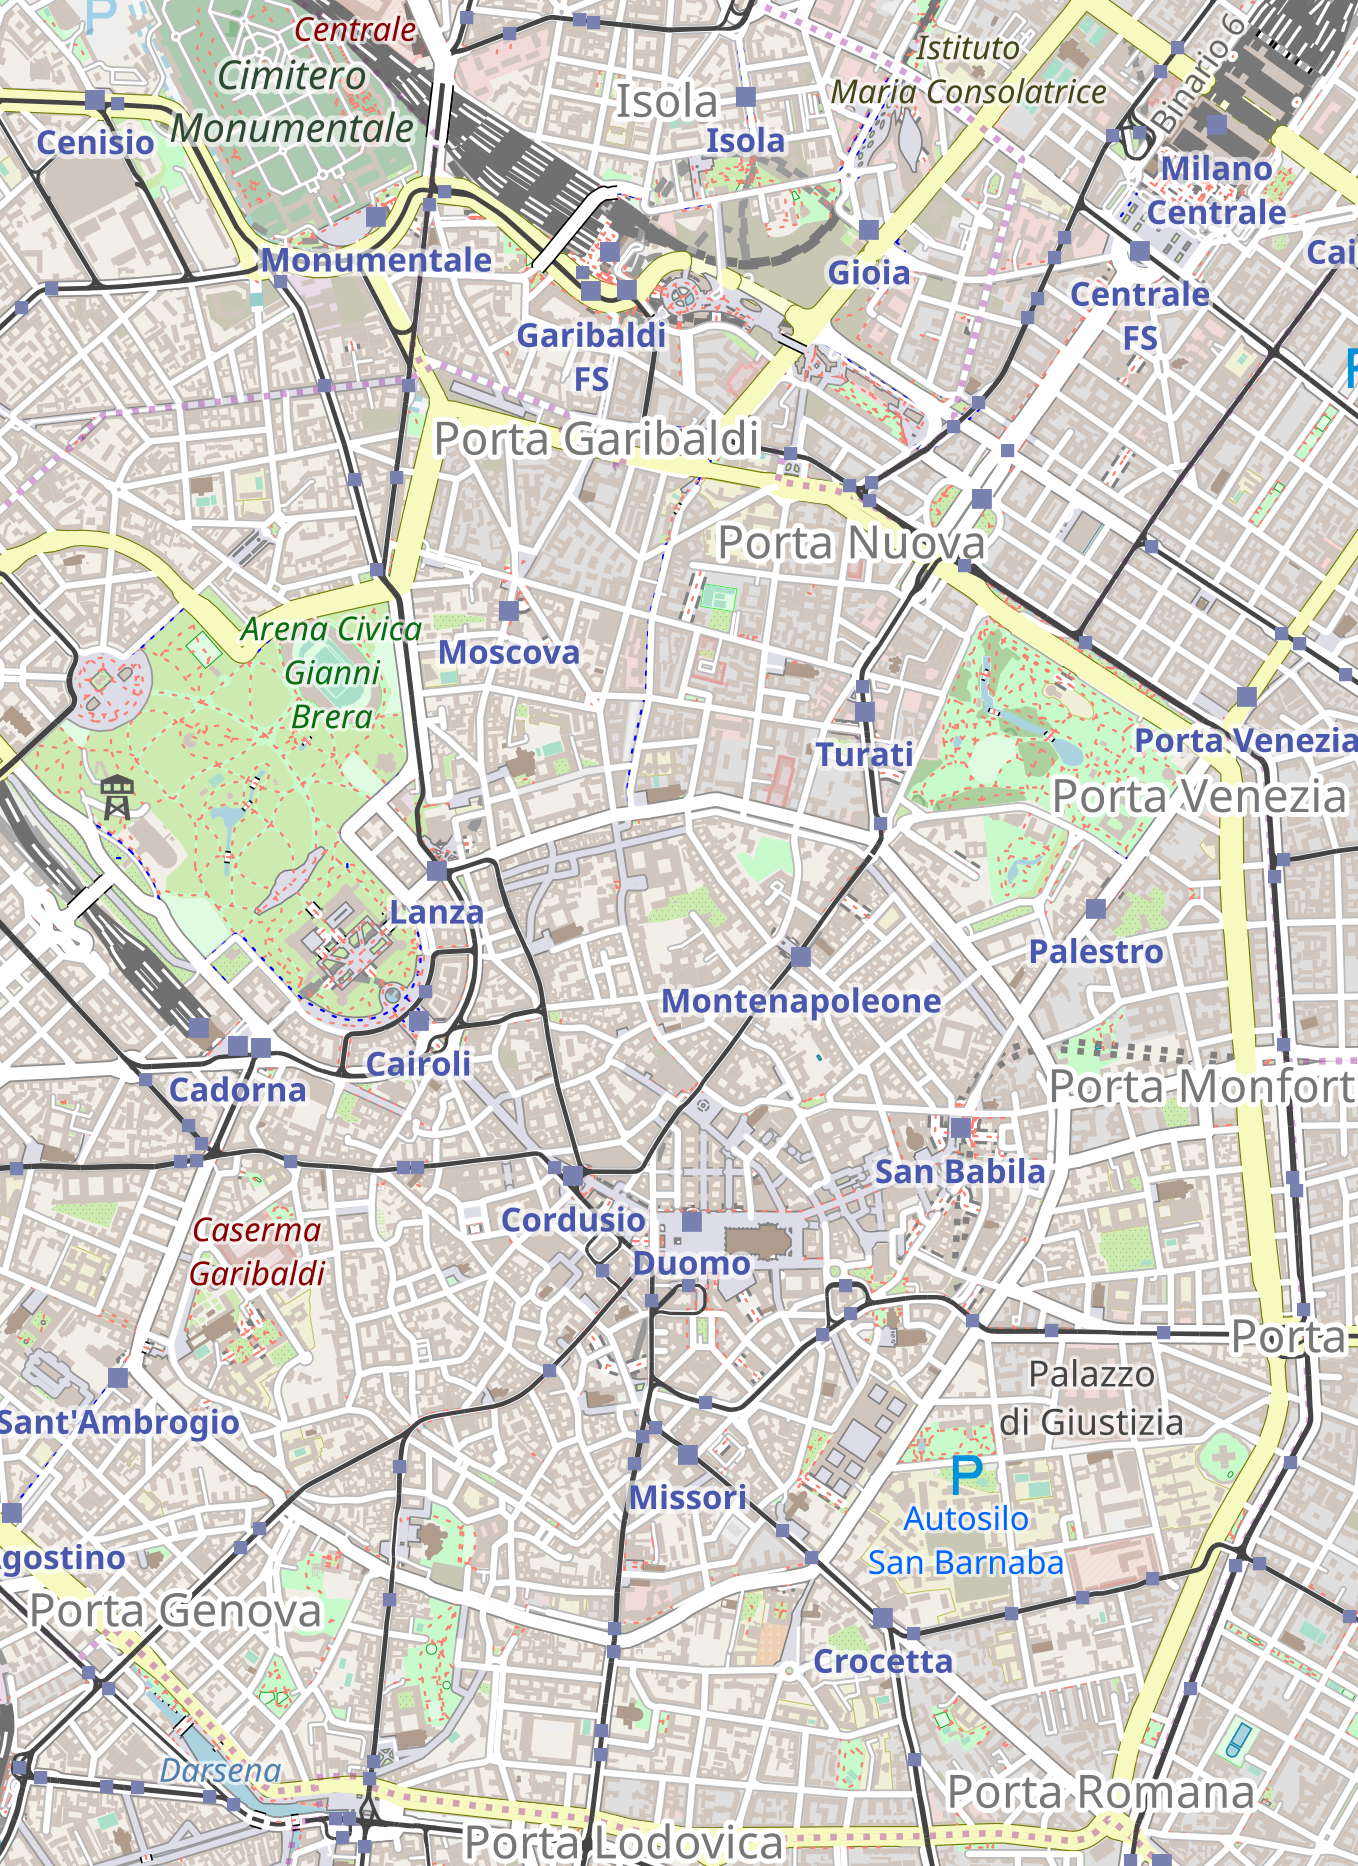
\includegraphics[width=115mm]{images-print/city-left.png}%
  }%
]{cityleft}
\DeclareNewLayer[background,%
  oddpage,
  width=115mm,%
  height=158mm,%
  hoffset=5mm,
  voffset=5mm,
  contents={%
    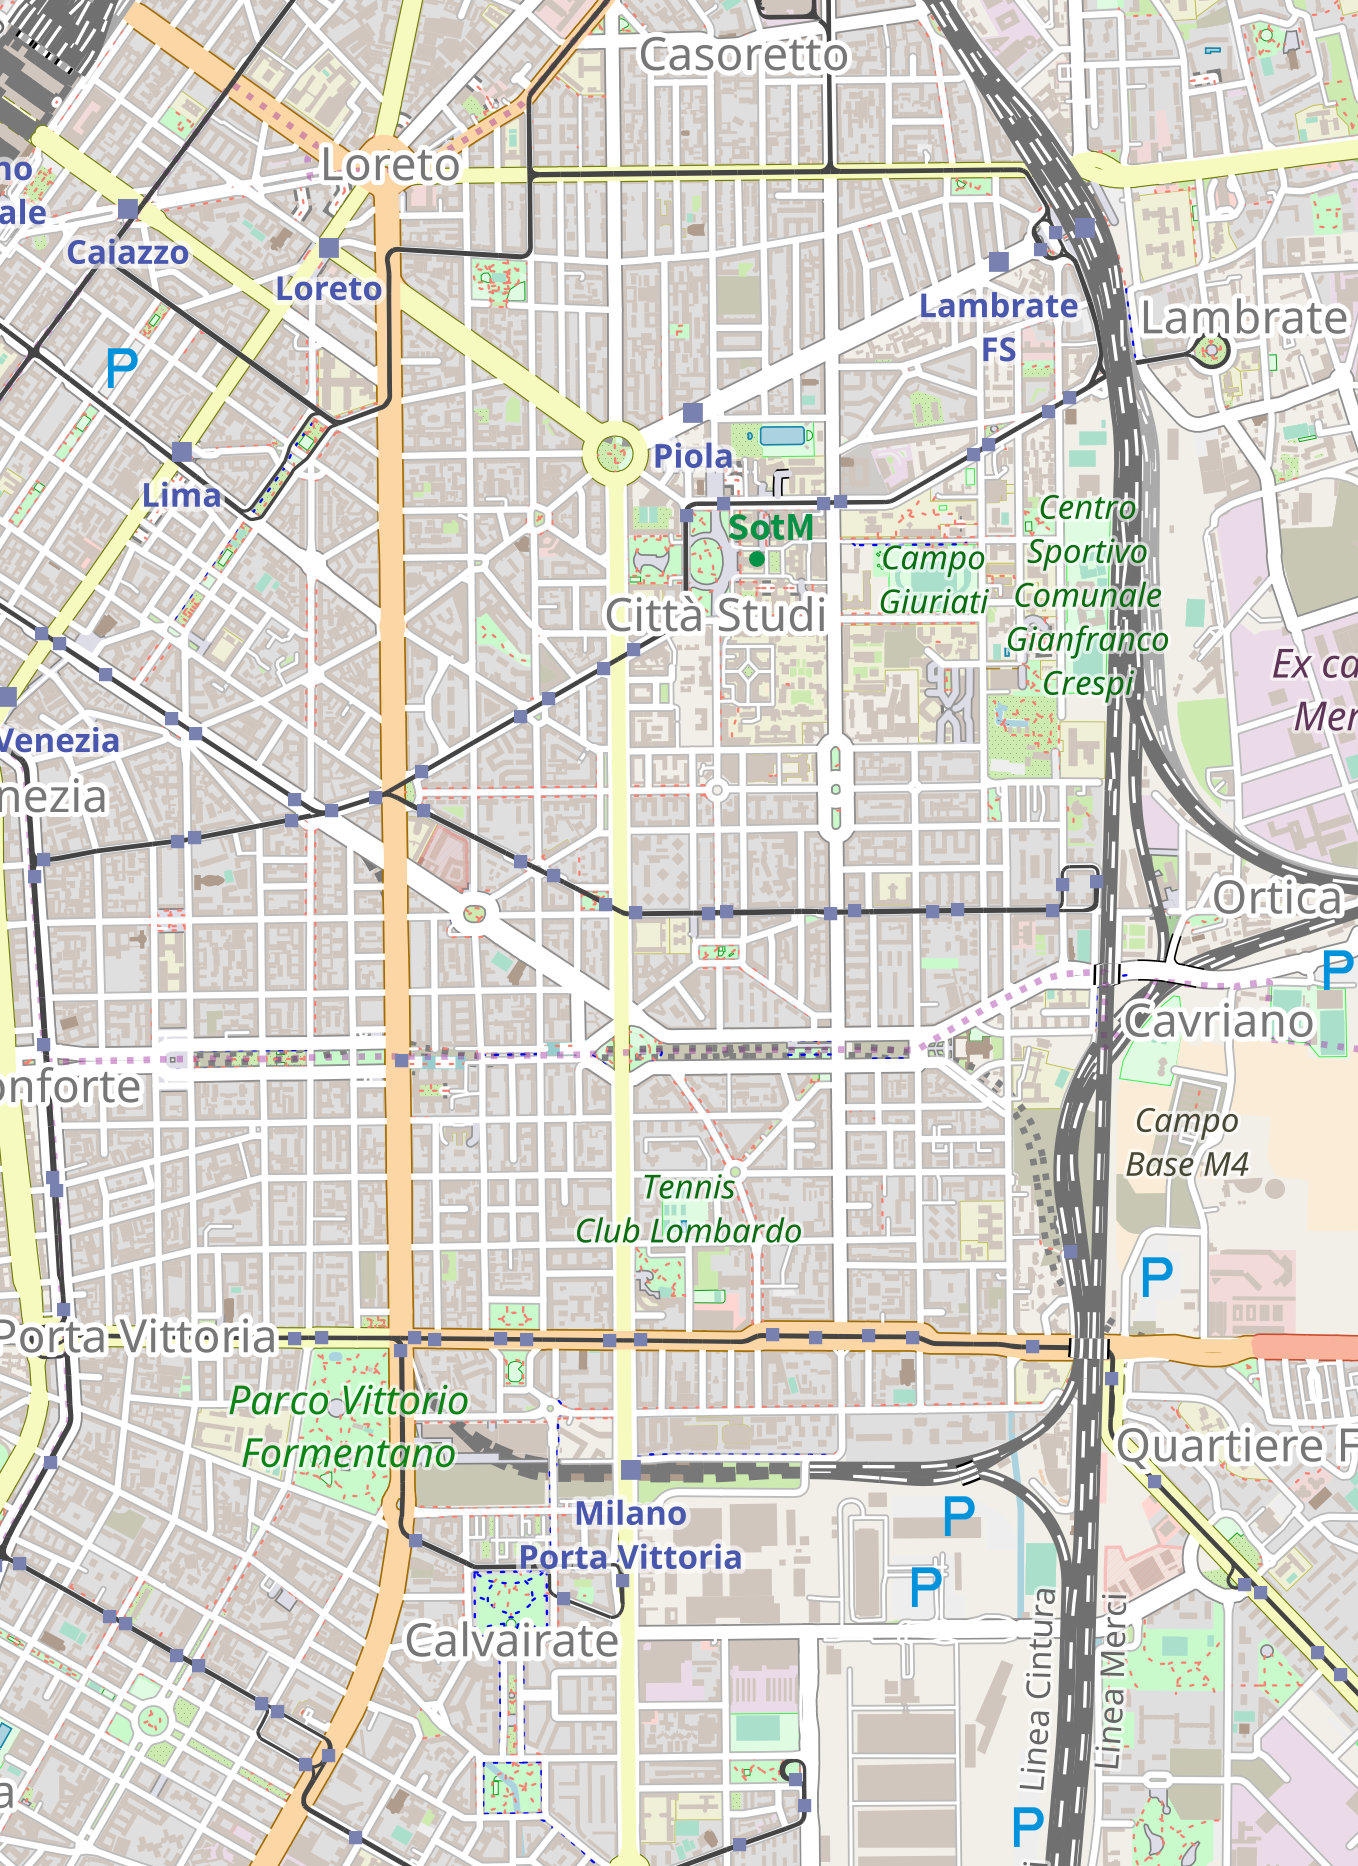
\includegraphics[width=115mm]{images-print/city-right.png}%
  }%
]{cityright}
\newpairofpagestyles{citymap}{}
\AddLayersAtBeginOfPageStyle{citymap}{cityleft}
\AddLayersAtBeginOfPageStyle{citymap}{cityright}
\AddLayersAtBeginOfPageStyle{citymap}{cropmarksevery}

% back cover
\DeclareNewLayer[background,%
  width=115mm,%
  height=158mm,%
  hoffset=5mm,
  voffset=5mm,
  contents={%
    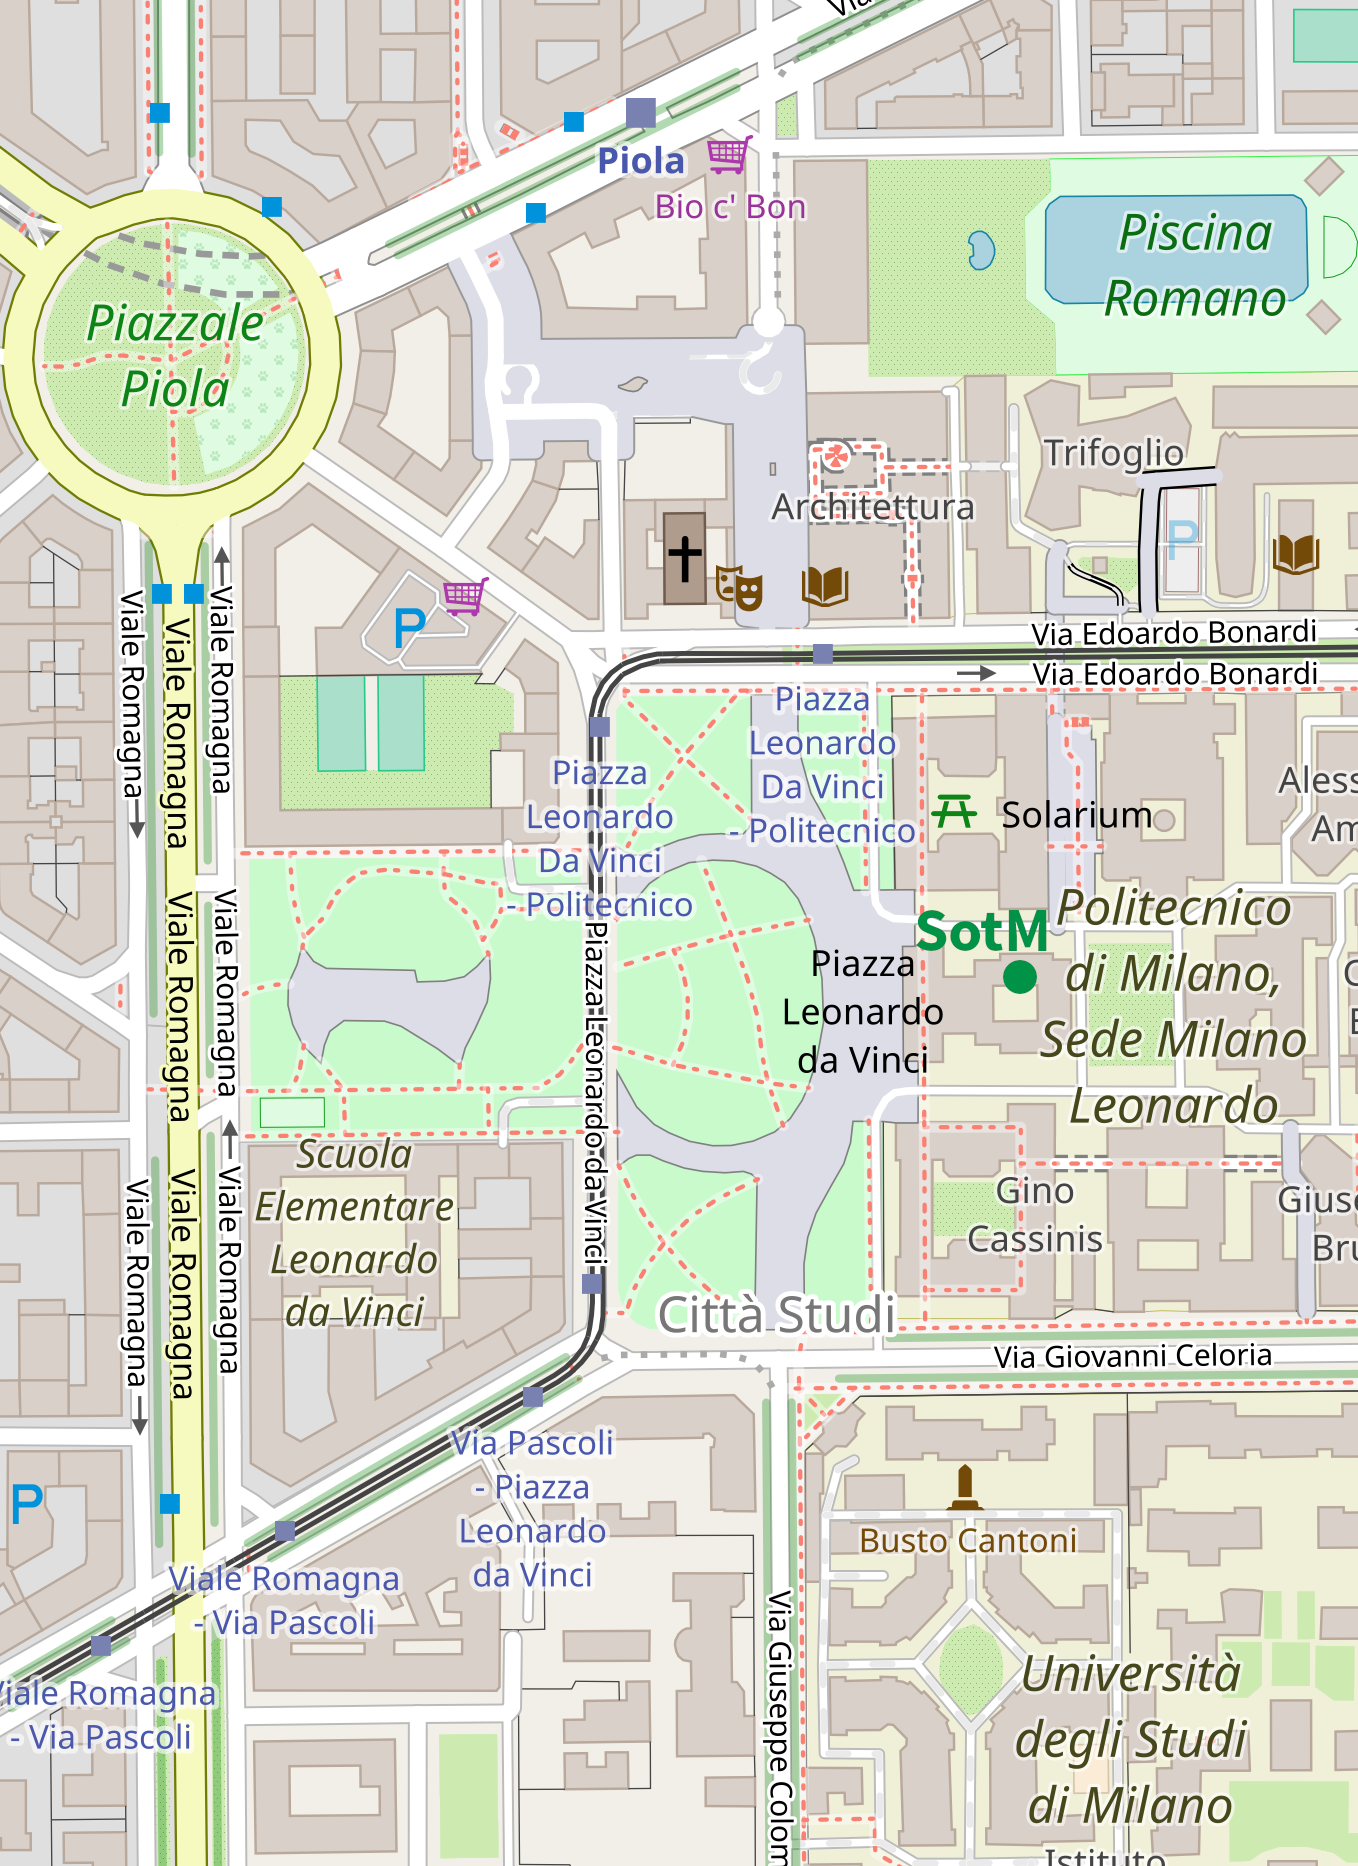
\includegraphics[width=115mm]{images-print/campus.png}%
  }%
]{campus}
\definecolor{sotmgreen}{cmyk}{1.0 0.0 0.52 0.43}
\usetikzlibrary{positioning}
\DeclareNewLayer[background,%
  width=115mm,%
  height=158mm,%
  hoffset=79mm,
  voffset=95mm,
  contents={%
    \begin{tikzpicture}[x=1mm, y=1mm]
      \node[inner sep=1.5mm, circle, fill, sotmgreen] (n1) {};
      \node[above=1mm of n1] {\Large \textcolor{sotmgreen}{\textbf{SotM}}};
    \end{tikzpicture}
  }%
]{campussotmmarker}
\newpairofpagestyles{backcover}{}
\AddLayersAtBeginOfPageStyle{backcover}{campussotmmarker}
\AddLayersAtBeginOfPageStyle{backcover}{campus}
\AddLayersAtBeginOfPageStyle{backcover}{campus}
\AddLayersAtBeginOfPageStyle{backcover}{cropmarksevery}


\begin{document}
 
\pagestyle{cropmarksstyle}
\begin{titlepage}
  \thispagestyle{titlestyle}
  \null
\end{titlepage}
\pagestyle{cropmarksstyle}

\selectlanguage{english}
\section*{Content}

\vspace*{0.35em}%
\noindent Welcome\dotfill \pageref{welcome}

\vspace*{0.35em}%
\noindent Scholarships \dotfill \pageref{scholarships}

\vspace*{0.35em}%
\noindent Getting around in Milan \dotfill \pageref{getting-around}

\vspace*{0.35em}%
\noindent Code of Conduct \dotfill \pageref{coc}

\vspace*{0.35em}%
\noindent Saturday \dotfill \pageref{saturday}

\vspace*{0.35em}%
\noindent Sunday \dotfill \pageref{sunday}

\vspace*{0.35em}%
\noindent Monday \dotfill \pageref{monday}

\vspace*{0.35em}%
\noindent Lightning talks \dotfill \pageref{lightning-talks}

\vspace*{0.35em}%
\noindent OpenStreetMap Foundation \dotfill \pageref{osmf}

\vspace*{0.35em}%
\noindent Thanks \dotfill \pageref{thanks}

\vspace*{0.35em}%
\noindent Sponsors \dotfill \pageref{sponsors}

\vspace*{0.35em}%
\noindent Maps \dotfill \pageref{maps}

\vspace*{0.35em}%
\noindent Legal notice \dotfill \pageref{legal}

\vfill
\noindent
Hashtag: \#sotm

\vspace*{0.8em}%
\noindent
The general emergency telephone number in Italy is \textbf{112}.
\vfill

\small{
\noindent
  \** Sessions in this room will not be recorded on video.\\
  \**\** This session will not be recorded on video.
}\normalsize


\newpage

\newpage
\enlargethispage{1\baselineskip}
\section*{Welcome to Milan and State of the Map 2018} \label{welcome}
This booklet provides you essential information
about the conference, the location and the schedule.  We are proud of the participation of the
OpenStreetMap community and our rich program but there is even more!  Please do get involved and
take advantage of the off-schedule sessions, discussions and spaces.

\paragraph*{Help desk} \label{welcome-helpdesk}
You already know the registration desk, located on the ground floor (Building 3, same as the whole
conference). It is also your port of call if you need support or help. We are listening to every
question, report and comment related to the event, the code of conduct (page~\pageref{coc}) or any
aspect of the organisation.

\paragraph*{Programme}
You can find the diverse programme on page~\pageref{saturday}ff. Full abstracts of all talks are available at https://2018.stateofthe\\map.org/program

\paragraph*{More than just talks} \label{welcome-location}
Room S.1.6 is available during the whole conference as free and open space offering chairs and tables
to talk to each other, work on your projects or just relax. Rooms S.1.3 (Saturday and Monday only) and S.1.4 are available for
self-organised sessions.  Please come to the welcome desk next to De Donato hall to announce your session.

\paragraph*{Sponsors} \label{welcome-sponsors}
We would like to thank our sponsors for making this event possible and for their support to the
OpenStreetMap Foundation.
\newpage

\newpage
\section*{Scholarships}
\label{scholarships}
\pagestyle{cropmarksstyle}

The OpenStreetMap Foundation is delighted to be able to provide scholarships to a number of
recipients from Europe, the Americas, Africa and Asia:

\RaggedRight
\begin{multicols}{2}
  Alsino Skowronnek\\
  Arnalie Faye Vicario\\
  Austin Zhu\\
  Céline Jacquin\\
  Cidália Costa Fonte\\
  Dennis Irorere\\
  Geoffrey Kateregga\\
  Kshitiz Khanal\\
  Laura Mugeha\\
  Montseng Moeti\\
  Natália da Silveira Arruda\\
  Rebecca Firth\\
  Remígio Chilaule\\
  Sebastian Meier\\
  Tasauf A Baki Billah\\
  Timofey Subbotin\\
  Wulansari Khairunisa\\
\end{multicols}
\justifying

The OpenStreetMap Foundation was not the only organisation granting scholarships. Les Libres
Geographes (with the overall support of Organisation Internationale de la Francophonie) facilitates five and Wikimedia Deutschland three scholarships over their own scholarship programmes.

\input{getting-around}
\newpage
\renewcommand{\arraystretch}{1.4}
%\section*{Saturday Schedule}
\label{saturday}
\pagestyle{saturday-table}
\newgeometry{
  paperwidth=125mm,
  paperheight=168mm,
  portrait,
  top=22mm,
  inner=20mm, % usually 22mm
  outer=17mm, % usually 20mm
  bottom=20mm,
  headsep=3mm,
  footskip=7mm
}
\setpagebackground
\noindent\begin{landscape}
  \begin{center}
    \noindent\begin{tabular}{Z{0.75cm}Z{10.83cm}}
      \cellcolor{commongray}
      &
      \multicolumn{1}{c}{
        \cellcolor{deDonato}
        De Donato
      }
      \tabularnewline
      \cellcolor{commongray}
      09:30
      \talk{Welcome}{}
      \tabularnewline
      \cellcolor{commongray}
      10:00
      \talk{\emph{Keynote} OpenStreetMap—now and into the future}{Kate Chapman, Heather Leson}
      \tabularnewline
      \rowcolor{commongray}
    \end{tabular}
  
    % remove white gap
    \vspace{-0.1\baselineskip}
    \enlargethispage{1\baselineskip}
    \noindent\begin{tabular}{Z{0.75cm}Z{5.20cm}Z{5.200cm}}
      \cellcolor{commongray}
      &
      \multicolumn{1}{c}{\cellcolor{deDonato} De Donato}
      & \multicolumn{1}{c}{\cellcolor{two} S.0.2}
      \tabularnewline
      \cellcolor{commongray}
      10:30
      \talk{Can we validate every change on OpenStreetMap?}{Lukas Martinelli}
      \talk{Making maps without databases}{Thomas Skowron}
      \tabularnewline
      \rowcolor{commongray}
      11:00 & \multicolumn{2}{c}{%
        \parbox[c]{18pt}{%
          \includegraphics[height=10pt]{cafe}%
        }
        break} \tabularnewline
    \end{tabular}
  
    % remove white gap
    \vspace{-0.1\baselineskip}
    \noindent\begin{tabular}{Z{0.75cm}Z{3.330cm}Z{3.330cm}Z{3.330cm}}
      \cellcolor{commongray}
      & \multicolumn{1}{c}{\cellcolor{deDonato} De Donato}
      & \multicolumn{1}{c}{\cellcolor{two} S.0.3}
      & \multicolumn{1}{c}{\cellcolor{four} S.1.5*}
      \tabularnewline
      \cellcolor{commongray}
      11:30
      \talk{Interpreting imagery for OpenStreetMap}{Chad Blevins}
      \talk{OpenMapTiles--- \mbox{vector} tiles from \mbox{OpenStreetMap}}{Petr Pridal, Jiri Komarek}
      \talk{Qt to create maps}{Paolo Angelelli}
      \tabularnewline
    \end{tabular}
  \end{center}

  \begin{center}
    \renewcommand{\arraystretch}{1.3}
    \noindent\begin{tabular}{Z{0.75cm}Z{3.330cm}Z{3.330cm}Z{3.330cm}}
      \cellcolor{commongray}
      & \multicolumn{1}{c}{\cellcolor{deDonato} De Donato}
      & \multicolumn{1}{c}{\cellcolor{two} S.0.3}
      & \multicolumn{1}{c}{\cellcolor{four} S.1.5*}
      \tabularnewline
      \cellcolor{commongray}
      12:00
      \talk{Advertising mapping--- using OpenStreepMap for the protection of landscape}{Paul Desgranges}
      %\talk{Advertising mapping}{Paul Desgranges}
      \talk{Large scale deep learning for map making}{Alina Negreanu, Bogdan Gliga}
      \longTalk{2}{\emph{Workhop (60 min)}\linebreak Field mapping tools and technologies}{Paul Uithol}
      \tabularnewline
      \cellcolor{commongray}
      12:30
      \talk{An excursion in to the world of OSM tagging presets}{Simon Poole}
      \talk{How deep learning could help to improve OSM data quality?}{Oliver Courtin}
      \tabularnewline
      \rowcolor{commongray}
      13:00 & \multicolumn{3}{c}{%
      \parbox[c]{18pt}{%
        \includegraphics[height=10pt]{restaurant}%
      }
      lunch} \tabularnewline
      \rowcolor{commongray}
      14:00
      & \multicolumn{3}{c}{
        \parbox[c]{18pt}{%
          \includegraphics[height=10pt]{photo}%
        }
        photo
      }
      \tabularnewline
    \end{tabular}
  \end{center}
    
  \begin{center}
    \renewcommand{\arraystretch}{1.3}
    \noindent\begin{tabular}{Z{0.75cm}Z{3.330cm}Z{3.330cm}Z{3.330cm}}
      \cellcolor{commongray}
      & \multicolumn{1}{c}{\cellcolor{deDonato} De Donato}
      & \multicolumn{1}{c}{\cellcolor{two} S.0.3}
      & \multicolumn{1}{c}{\cellcolor{four} S.1.5*}
      \tabularnewline
      \cellcolor{commongray}
      14:10
      \talk{Addressing addresses}{Sarah Hoffmann}
      \talk{The Belgian perspective to building OpenStreetMap community}{Ben Abelshausen, Joost Schouppe}
      %\talk{Belgian perspective to building OSM community}{Ben Abels\-hausen, Joost Schouppe}
      \talk{Lightning talks 1}{}
      \tabularnewline
      \cellcolor{commongray}
      14:40
      \talk{2, 4, 6, 8, Here's how we interpolate}{Julian Simioni}
      \talk{A new approach to garner prolific contribution in OpenStreetMap}{Kshitiz Khanal}
      %\talk{New approach to garner prolific contribution in OSM}{Kshitiz Khanal}
      \longTalk{2}{\emph{Workshop (60 min)}\linebreak The LWG presents: GDPR implementation for OSM}{Kathleen Lu}
      \tabularnewline
      \cellcolor{commongray}
      15:10
      \talk{OsmAnd making live maps update}{Victor Shcerb}
      \talk{Building up the \mbox{Microsoft} Open Maps Team}{Osin Herriott}
      \tabularnewline
      \rowcolor{commongray}
      15:40
      & \multicolumn{3}{c}{%
      \parbox[c]{18pt}{%
        \includegraphics[height=10pt]{cafe}%
      }
      break} \tabularnewline
    \end{tabular}
  \end{center}
    
  \begin{center}
    \renewcommand{\arraystretch}{1.3}
    \noindent\begin{tabular}{Z{0.75cm}Z{3.330cm}Z{3.330cm}Z{3.330cm}}
      \cellcolor{commongray}
      & \multicolumn{1}{c}{\cellcolor{deDonato} De Donato}
      & \multicolumn{1}{c}{\cellcolor{two} S.0.3}
      & \multicolumn{1}{c}{\cellcolor{four} S.1.5*}
      \tabularnewline
      \cellcolor{commongray}
      16:10
      \talk{Lies, damned lies, and OSM statistics}{Frederik Ramm}
      \talk{Verifying our edits}{Bogdan Petrea, Armin Gheorghina}
      \talk{Corporate cartography: How the sausage gets made}{Paul Norman}
      \tabularnewline
      \cellcolor{commongray}
      16:40
      \talk{An innovative approach to support OSM data generation}{Emanuela Mihut}
      \talk{Mapping competition with focus on quality: lesson learned}{Yantisa Akhadi}
      \longTalk{2}{\emph{Workshop (60 min)}\linebreak Open Gender Monologues}{Heather Leson}
      \tabularnewline
      \cellcolor{commongray}
      17:10
      \talk{Pinpointing the power grid}{Sajjad Anwar}
      \talk{Improving OSMCha for the community}{Wille Marcel Lima Malheiro}
      &
      \tabularnewline
      \rowcolor{commongray}
      17:40
      & \multicolumn{3}{c}{%
        \parbox[c]{18pt}{%
          \includegraphics[height=10pt]{community_centre}%
        }
        Get involved in the OSM Foundation! (until 18:30)%
      }
      \tabularnewline
    \end{tabular}
  \end{center}
\end{landscape}
\renewcommand{\arraystretch}{1.0}
\restoregeometry

\newpage
\renewcommand{\arraystretch}{1.4}
\renewcommand{\conferenceDay}{\sunday}
\setpagebackground
\pagestyle{sunday-table}
\newgeometry{
  paperwidth=125mm,
  paperheight=168mm, 
  portrait,
  top=22mm,
  inner=20mm, % usually 22mm
  outer=17mm, % usually 20mm
  bottom=20mm,
  headsep=3mm,
  footskip=7mm
}
\noindent\begin{landscape}
  %\section*{Sessions on Sunday}
  \label{sunday}
  \noindent\begin{center}
    \noindent\begin{tabular}{Z{0.75cm}Z{2.0cm}Z{2.2cm}Z{3.40cm}Z{2.0cm}}
    %\noindent\begin{tabular}{Z{0.75cm}Z{2.0cm}Z{2.0cm}Z{2.8cm}Z{2.0cm}}
      \cellcolor{commongray}
      & \multicolumn{1}{c}{\cellcolor{deDonato} De Donato}
      & \multicolumn{1}{c}{\cellcolor{two} S.0.3}
      & \multicolumn{1}{c}{\cellcolor{academic} S.1.3}
      & \multicolumn{1}{c}{\cellcolor{four} S.1.5}
      \tabularnewline
      \cellcolor{commongray}
      09:30
      \talk{Alternative perspectives through artistic interpretations}{Sebastian Meier et\,al.}
      \talk{What's up with the public transport}{Ilya Zverev}
      \talk{Coordinating improved communication between the academic and OSM communities}{Peter Mooney et\,al.}
      \tabularnewline
      \cellcolor{commongray}
      10:00
      \talk{Lightning talks 2}{}
      \talk{Network for transport open data}{Céline Jacquin}
      \talk{Surveying OSM contributors: Learning from the community}{Zoe Gardner, Peter Mooney}
      \talk{Thematic mapping with emojis}{Erik Escoffier}
      \tabularnewline
      \cellcolor{commongray}
      10:30
      \talk{Lightning talks 3}{}
      \talk{Solving routing problems with OSM and VROOM}{Julien Coupey}
      %\talk{Solving vehicle routing problems with OpenStreetMap and VROOM}{Julien Coupey}
      \talk{Slum health mapping as catalyst for a collaborative aganda for research, practice, local~\dots}{João Porto de Albuquerque et\,al.}
      %\talk{Slum health mapping as catalyst for a collaborative agenda for research, practice, local citizens and volunteers}{João Porto de Albuquerque et\,al.}
      \talk{Open\-Street\-Map My \mbox{Business}}{Stefan Keller}
      \tabularnewline
    \end{tabular}
  \end{center}
  \begin{center}
    \noindent\begin{tabular}{Z{0.75cm}Z{2.0cm}Z{2.2cm}Z{3.4cm}Z{2.0cm}}
    %\noindent\begin{tabular}{Z{0.75cm}Z{2.0cm}Z{2.0cm}Z{2.8cm}Z{2.0cm}}
      \cellcolor{commongray}
      & \multicolumn{1}{c}{\cellcolor{deDonato} De Donato}
      & \multicolumn{1}{c}{\cellcolor{two} S.0.3}
      & \multicolumn{1}{c}{\cellcolor{academic} S.1.3}
      & \multicolumn{1}{c}{\cellcolor{four} S.1.5}
      \tabularnewline
      \rowcolor{commongray}
      11:00
      & \multicolumn{4}{c}{%
      \parbox[c]{24pt}{%
        \includegraphics[height=10pt]{cafe}%
      }
      break}
      \tabularnewline
      \cellcolor{commongray}
      11:30
      \talk{OSM and the European agenda}{Vlado Cetl}
      \talk{The use of OSM in public transport in Helsinki, Finland}{Markku Huotari}
      %\talk{The use of OSM in public transport in Helsinki}{Markku Huotari}
      %\talk{Human-Centered Data Science and OSM: Contributor-Centric OpenStreetMap Analysis Infrastructure}{Anderson}
      \talk{Human-centered data science and OSM: contributor-centric OSM analysis infrastructure}{Jennings Anderson}
      \talk{Some location intelligence from OSM}{Jaak Laineste}
      \tabularnewline
      \cellcolor{commongray}
      12:00
      \longTalk{2}{\emph{Panel (60 min)}\linebreak Sustainability of OSM mapping projects}{Erica Hagen}
      \talk{Printing OSM maps}{Hartmut Holzgraefe}
      %\talk{Intrinsic assessment of the temporal accuracy, up-to-dateness, lineage and thematic accuracy of OpenStreetMap}{Frassinelli et\,al.}
      \talk{Intrinsic assessment of the temporal accuracy, up-to-dateness, lineage and thematic accuracy}{Francesco Frassinelli et\,al.}
      \longTalk{2}{\emph{Workshop (60 min)}\linebreak Humans and machines mapping \mbox{together}}{Zhuangfang NaNa Yi}
      \tabularnewline
      \cellcolor{commongray}
      12:30
      &
      \talk{Osmose-QA and validation with JOSM}{Fr\'{e}d\'{e}ric Rodrigo}
      %\talk{Osmose-QA \& Common validation with JOSM}{Fr\'{e}d\'{e}ric Rodrigo}
      \talk{Comprehensive OSM history data analyses~-- for and with the OSM community}{Michael Auer et\,al.}
      &
    \end{tabular}
  \end{center}
  \begin{center}
    \noindent\begin{tabular}{Z{0.75cm}Z{2.0cm}Z{2.0cm}Z{3.6cm}Z{2.0cm}}
    %\noindent\begin{tabular}{Z{0.75cm}Z{2.0cm}Z{2.0cm}Z{2.8cm}Z{2.0cm}}
      \cellcolor{commongray}
      & \multicolumn{1}{c}{\cellcolor{deDonato} De Donato}
      & \multicolumn{1}{c}{\cellcolor{two} S.0.3}
      & \multicolumn{1}{c}{\cellcolor{academic} S.1.3}
      & \multicolumn{1}{c}{\cellcolor{four} S.1.5}
      \tabularnewline
      \rowcolor{commongray}
      13:00
      & \multicolumn{4}{c}{%
        \parbox[c]{24pt}{%
          \includegraphics[height=10pt]{restaurant}%
        }
      lunch}
      \tabularnewline
      \cellcolor{commongray}
      14:00
      \longTalk{2}{\emph{Panel (60 min)}\linebreak The road towards diversity in OSM still needs to be mapped}{Céline Jacquin}
      \talk{Navigating  with OSM in Bangladesh}{Tasauf A Baki Billah}
      %\talk{Pathao: Navigating  with OSM in Bangladesh while Community blends in with Corporate}{Tasauf A Baki Billah}
      \talk{An innovative approach to support OSM data generation}{Emanuela Mihut et\,al.}
      \longTalk{2}{\emph{Workshop (60 min)}\linebreak Exploring OSM's history using the Ohsome data analytics platform}{Martin Raifer et\,al.}
      \tabularnewline
      \cellcolor{commongray}
      14:30
      &
      \talk{Flying ferries and moving pavements?}{Guillaume Rischard}
      %\talk{Flying ferries and moving pavements? Pedestrian routing on rare modes of transport}{Guillaume Rischard}
      \talk{Investigating the mapping process after disasters: Osm\-Event\-Analyst and its application for the 2016 Italian earthquakes}{L. Delucchi, M. Minghini}
      &
      \tabularnewline
      \cellcolor{commongray}
      15:00
      \talk{Lightning talks 4}{}
      \talk{CityZen}{Redon Skikuli}
      %\talk{Privacy aware city navigation with CityZen app}{Redon Skikuli}
      \talk{Areas-of-Interest for OpenStreetMap with big spatial data analytics}{Stefan Keller}
      \talk{IT backend of the OSM community}{Timofey}
      %\talk{IT backend of the OpenStreetMap community}{Timofey}
      \tabularnewline
    \end{tabular}
  \end{center}
  \begin{center}
    \noindent\begin{tabular}{Z{0.75cm}Z{2.0cm}Z{2.0cm}Z{3.6cm}Z{2.0cm}}
    %\noindent\begin{tabular}{Z{0.75cm}Z{2.0cm}Z{2.0cm}Z{2.8cm}Z{2.0cm}}
      \cellcolor{commongray}
      & \multicolumn{1}{c}{\cellcolor{deDonato} De Donato}
      & \multicolumn{1}{c}{\cellcolor{two} S.0.3}
      & \multicolumn{1}{c}{\cellcolor{academic} S.1.3}
      & \multicolumn{1}{c}{\cellcolor{four} S.1.5}
      \tabularnewline
      \rowcolor{commongray}
      15:30
      & \multicolumn{4}{c}{%
      \parbox[c]{24pt}{%
        \includegraphics[height=10pt]{cafe}%
      }
      break}
      \tabularnewline
      \cellcolor{commongray}
      16:00
      \talk{A tale of two (mapping) cities}{A. Skow\-ron\-nek, M. Feretti}
      %\talk{A tale of two (mapping) cities}{Alsino Skow\-ron\-nek, Mi\-chele Ferretti}
      \talk{Lightning talks 5}{}
      \talk{Potential and limitation of using OSM data for the creation/validation of land use/cover maps}{Cidália C. Fonte}
      \talk{A community-driven non-profit mapping agency}{Ben Abelshausen}
      \tabularnewline
      \cellcolor{commongray}
      16:30
      \talk{OSM Community Grants: sharing experiences}{Rebecca Firth}
      \talk{Lightning talks 6}{}
      \talk{The challenges and issues associated with a natural resource mapping framework based upon OSM}{Chris Emberson et\,al.}
      \longTalk{2}{\emph{Workshop (60 min)}\linebreak Navigation mapping workshop}{Kajari Ghosh}
      \tabularnewline
      \cellcolor{commongray}
      17:00
      \talk{Working with the comunity}{Ryan Peterson}
      \talk{Lightning talks 7}{}
      \talk{Using OpenStreetMap to model bicycle traffic in an agent-based transport simulation}{D. Ziemke, S. Metzler}
      &
      \tabularnewline
    \end{tabular}
  \end{center}
\end{landscape}
\renewcommand{\arraystretch}{1.0}
\justifying
\restoregeometry
\setpagebackground

\newpage
\renewcommand{\arraystretch}{1.4}
\renewcommand{\conferenceDay}{\sunday}
\setpagebackground
\pagestyle{monday-table}
\newgeometry{
  paperwidth=125mm,
  paperheight=168mm, 
  portrait,
  top=22mm,
  inner=20mm, % usually 22mm
  outer=17mm, % usually 20mm
  bottom=20mm,
  headsep=3mm,
  footskip=7mm
}
\noindent\begin{landscape}
  %\section*{Sessions on Monday}
  \label{monday}
  \noindent\begin{center}
    \noindent\begin{tabular}{Z{0.75cm}Z{3.330cm}Z{3.330cm}Z{3.330cm}}
      \cellcolor{commongray}
      & \multicolumn{1}{c}{\cellcolor{deDonato} De Donato}
      & \multicolumn{1}{c}{\cellcolor{two} S.0.3}
      & \multicolumn{1}{c}{\cellcolor{four} S.1.5*}
      \tabularnewline
      \cellcolor{commongray}
      09:30
      \talk{Completing the map with street-level \mbox{imagery}}{Christopher Beddow}
      \talk{Road Completion in Belgium--mapping and verifying all the roads}{Ben Abelshausen}
      \talk{Lightning talks 8}{}
      \tabularnewline
      \cellcolor{commongray}
      10:00
      \talk{Pic4Review: fun OSM editing based on street pictures}{Adrien Pavie}
      \talk{Going to production with OpenStreeetMap at Microsoft}{Jubal Harpster}
      \longTalk{3}{\emph{Workshop (60 min)}\linebreak Building your OSM web app in minutes with vector tiles}{Lukas Martinelli, Jinal Foflia}
      \tabularnewline
      \cellcolor{commongray}
      10:30
      \talk{Form and map based mobile tool for survey and validation}{Kuo-Yu slayer Chuang}
      %\talk{Form \& Map based Mobile OSM Tool for Field Survey and Validation}{Kuo-Yu slayer Chuang}
      \talk{Switch2OSM---a real enterprise context case study}{Andrea Capata}
      &
      \tabularnewline
      \rowcolor{commongray}
      11:00
      & \multicolumn{3}{c}{%
        \parbox[c]{24pt}{%
          \includegraphics[height=10pt]{cafe}%
        }
      break}
      \tabularnewline
    \end{tabular}
  \end{center}
  \noindent\begin{center}
    \noindent\begin{tabular}{Z{0.75cm}Z{3.330cm}Z{3.330cm}Z{3.330cm}}
      \cellcolor{commongray}
      & \multicolumn{1}{c}{\cellcolor{deDonato} De Donato}
      & \multicolumn{1}{c}{\cellcolor{two} S.0.3}
      & \multicolumn{1}{c}{\cellcolor{four} S.1.5*}
      \tabularnewline
      \cellcolor{commongray}
      11:30
      %\talk{The new Wheelmap}{Svenja Heinecke}
      \talk{The new Wheelmap: Joining forces in accessibility mapping---feat.: "I Wheel Share"}{Svenja Heinecke}
      \talk{Making bot edits safe and acceptable}{Yuri Astrakhan}
      \longTalk{2}{\emph{Panel (60 min)}\linebreak OpenStreetMap and the future of transport}{Michele Ferretti}
      \tabularnewline
      \cellcolor{commongray}
      12:00
      \talk{Modding the OSM data model}{Jochen Topf}
      \talk{Robot Tracers---extraction and classification at scale using \& CNTK}{Nikola Trifunovic}
      &
      \tabularnewline
      \cellcolor{commongray}
      12:30
      \talk{Energy efficient routing with OSM}{Arndt Brenschede}
      \talk{Reaching out to vulnerable communities in Turkey}{Gülşah Eker}
      \talk{Attracting students with Google Summer of Code}{Peter Barth}
      \tabularnewline
      \rowcolor{commongray}
      13:00
      & \multicolumn{3}{c}{%
        \parbox[c]{24pt}{%
          \includegraphics[height=10pt]{restaurant}%
        }
      lunch}
      \tabularnewline
    \end{tabular}
  \end{center}
  \noindent\begin{center}
    \noindent\begin{tabular}{Z{0.75cm}Z{3.330cm}Z{3.330cm}Z{3.330cm}}
      \cellcolor{commongray}
      & \multicolumn{1}{c}{\cellcolor{deDonato} De Donato}
      & \multicolumn{1}{c}{\cellcolor{two} S.0.3}
      & \multicolumn{1}{c}{\cellcolor{four} S.1.5*}
      \tabularnewline
      \cellcolor{commongray}
      14:00
      \talk{Openrouteservice---route the world dynamically}{Nils Nolde}
      \talk{OSM enabled urban mobility services for the city of Yangon}{Robert Castelli}
      %\talk{OSM enabled urban mobility services for the city of Yangon, Myanmar}{Robert Castelli}
      \longTalk{2}{\emph{Workshop (60 min)}\linebreak Areas, routing, and diffs: Can we have something better than relations?}{Roland Olbricht}
      \tabularnewline
      \cellcolor{commongray}
      14:30
      \talk{Routing on rails with OpenStreetMap}{Michael Reichert}
      \talk{Community mapping for refugees in Uganda}{Geoffrey Kateregga}
      &
      \tabularnewline
      \cellcolor{commongray}
      15:00
      \talk{OSM at Facebook}{Drishtie Patel}
      \talk{Dronebirds are go!}{Taichi Furuhashi}
      \talk{Lightning talks 9}{}
      \tabularnewline
      \rowcolor{commongray}
      15:30
      & \multicolumn{3}{c}{%
        \parbox[c]{24pt}{%
          \includegraphics[height=10pt]{cafe}%
        }
      break}
      \tabularnewline
      \cellcolor{commongray}
      16:00
      \talk{Indonesia road \mbox{mapping}: Challenges and opportunities}{Wulansari Khairunisa}
      \talk{3D beyond buildings}{Tobias Knerr}
      \talk{Lightning talks 10}{}
      \tabularnewline
      \cellcolor{commongray}
      16:30
      \talk{Closing and OSM Awards ceremony}{}
      &
      &
    \end{tabular}
  \end{center}
\end{landscape}
\renewcommand{\arraystretch}{1.0}
\justifying
\restoregeometry
\setpagebackground

\newpage
\section*{Lightning Talks}
\label{lightning-talks}
\pagestyle{cropmarksstyle}
\enlargethispage{1\baselineskip}
\subsection*{Saturday 14:10 in S.1.5}
Nicole Martinelli: \emph{OpenStreetMaps for emergency prep: The view from San Francisco}\\
Daniel Mietchen: \emph{Wikimedia in disaster management and humanitarian aid: an overview}\\
Janet Chapman: \emph{Crowd2Map Tanzania---helping protect girls from FGM and empower rural communities}\\
Laura Mugeha: \emph{Role of mapping in achieving the Sustainable Development Goals (SDGs)}

\subsection*{Sudnay 10:00 in De Donato}
Instvan Vincze: \emph{Making a JOSM mapper's life simpler and easier}\\
ikushan: \emph{A new lightning fast .osm parser}\\
Bryan Housel: \emph{The state of the iD editor}\\
Simon Poole: \emph{State of Vespucci}

\subsection*{Sunday 10:30 in De Donato}
Remígio van Eys Chilaule: \emph{State of OSM in Mozambique: community presentation and on-going projects}\\
Alexandre Duclaux: \emph{Mapping Freetown’s distribution water network using OSM}\\
Javier Carranza Tresoldi: \emph{Third party data for the SDGs: What can openstreetmap bring to the table?}\\

\subsection*{Sunday 15:00 in De Donato}
Daniel Mietchen: \emph{Maps based on Wikidata queries}\\
Michael Spreng: \emph{FOSSGIS routing server}\\
Eugene Alvin Villar: \emph{OpenStreetMap and Wikimedia}\\
Stefan Eberlein: \emph{Providing OSM realtime extracts}

\subsection*{Sunday 16:00 in S.0.2}
Adriana Lazar: \emph{The Telenav Metrics Dashboard for OpenStreetMap}\\
Jinal Foflia: \emph{Where is the community?}\\
Ilya Zverv: \emph{Every day I'm mapping}\\
Thilo: \emph{Namespaces general description}

\subsection*{Sunday 16:30 in S.0.2}
Akhi Jetra: \emph{Brightest star among the crowd}\\
Massimiliano Bernabé: \emph{OpenStreetMap for the dyslexic}\\
Sandra Tabinas: \emph{Mental Health A-WHERE-ness PH: Mapping mental health resources in the Philippines}\\
Michael Bernhamou: \emph{Improving Public Policy with Geo-Statistics}

\subsection*{Sunday 17:00 in S.0.2}
Kristiina Kerge, Kadri Maripuu: \emph{MapIt -- Global trash hunt}\\
Balémta Aimée Sama: \emph{The face of OSM in Togo: data analysis and achievements}\\
Gregory Marler: \emph{State of the UK: 14 years of vision}\\
Arnalie Faye Vicario: \emph{Mapping A Paradise: Batanes, the Home of the Winds}

\subsection*{The stage is yours~\dots}

You are missing a talk? We have three slots (4 lightning talks each) left. Meet us at the welcome desk to
sign up.

New lightning talks and changes to the programme will be announced next to the welcome desk. Descriptions of the new lightning talks will be published on the OpenStreetMap wiki at \mbox{https://2018.stateofthemap.org/program}
% we will link to the wiki during the conference because that is easier to manage

\newpage
\section*{OpenStreetMap Foundation}
\label{osmf}
\pagestyle{osmf}
The OpenStreetMap Foundation is an
international non-profit organization
supporting, but not controlling,
OpenStreetMap. We are dedicated to
encouraging the growth, development and
distribution of free geospatial data and to
providing geospatial data for anyone to use
and share.

We need you as member. Members are vital
to the OSM Foundation -- to voice ideas
and shape the direction of the Foundation,
and support efforts of working groups. We
welcome all who support our goals to join us!

Find out more and join at osmfoundation.org
or join the session \emph{Get involved in the OpenStreetMap Foundation} on Saturday on 17:40.

\newpage
\section*{Thanks}
\label{thanks}
\pagestyle{cropmarksstyle}
%% short version:
% This conference would not have been possible with the huge support by a lot of volunteers. We would like to thank

Each year when we write this section we are reminded why OpenStreetMap is so great---it's the dedication
and passion of individuals who, when acting together, can achieve great things. This year is no
different. In fact we've been helped by a record number of people, many of whom are returning in
roles they supported in the previous year or two. The generosity of the following people have kept
us on track and each contribution, however small, moved us closer to our goal. Thank you.

State of the Map would not be possible without the support of the OpenStreetMap Foundation working
groups. Over the years we have worked with almost every working group, the Board, Advisory Board,
and of course our hosts of this year (Wikimedia Italia) are one of the OSMF Local Chapters. We 
encourage everyone to ask how they can help the groups---even a spare 10 minutes here and there can
make the difference.

\newlength{\volunteerSpace}
\setlength\volunteerSpace{0.8\baselineskip}
\RaggedRight
\begin{multicols}{2}
  \begin{small}
    \textbf{SotM Working Group}\\
    Benoît Fournier\\
    Christine Karch\\
    Gregory Marler\\
    Michael Reichert\\
    Mikel Maron\\
    Rob Nickerson

    \vspace{\volunteerSpace}
    \textbf{Local team}\\
    Alessandro Palmas\\
    Francesca Ussani\\
    Francesco Frassinelli\\
    Giovanna Ranci Ortigosa\\
    Marco Minghini\\
    Maria Antonia Brovelli\\
    Marta Erica Arosio\\

    \vspace{\volunteerSpace}
    \textbf{Academic selection committee}\\
    Amin Mobasheri\\
    Daniele Oxoli\\
    Cristian Consonni\\
    Darian Frajberg\\
    Frank Ostermann\\
    Gloria Bordogna\\
    Joost Schouppe\\
    Marco Minghini (lead)\\
    Maria Antonia Brovelli\\
    Monia Elisa Molinari\\
    Peter Mooney\\
    Piero Fraternali\\
    Rocio Nahime Torres\\
    Sofiane Abbar\\
    Stefan Keller\\
    Victoria Rautenbach\\
    Vyron Antoniou

    \vspace{\volunteerSpace}
    \textbf{Programme selection \mbox{committee}}\\
    Alessandro Palmas\\
    Andrew Wiseman\\
    Benoît Fournier\\
    Christine Karch\\
    Gregory Marler\\
    Mikel Maron\\
    Rob Nickerson\\
    Selene Yang\\
    Sidorela Uku\\
    Stefano Sabatini\\

    \vspace{\volunteerSpace}
    \textbf{Scholarship selection}\\
    Alessandro Palmas\\
    Christine Karch\\
    Gregory Marler\\
    Heather Leson\\
    Ilya Zverev\\
    Jóhannes Birgir Jensson\\
    Maurizio Napolitano\\
    Mikel Maron\\
    Rebecca Firth\\
    Rob Nickerson\\
    Selene Yang\\
    Sidorela Uku\\
    Stefano Sabatini\\

    \vspace{\volunteerSpace}
    \textbf{Volunteers at the event}\\
    Anna Rosati\\
    Aurelio Cilia\\
    Candan Eylül Kilsedar\\
    Cristian Consonni\\
    Daniele Oxoli\\
    Durgesh Nandini\\
    Fabio Cattaneo\\
    Federica Gaspari\\
    Gautam Kishore Shahi\\
    Lorenzo Stucchi\\
    Marco Brancolini\\
    Miloš Stojiljković\\
    Simone De Santis\\

    \vspace{\volunteerSpace}
    \textbf{Other}\\
    Angelica Braccia (logo design)\\
    Dorothea Kazazi (scholarship and admin support)\\
    Frederik Ramm (treasurer)\\
    Ilya Zverev (OSM Awards lead)\\
    Michael Montani (social media)\\
    Tom Hughes (ticket site)\\
  \end{small}
\end{multicols}
\justifying

\newpage
\pagestyle{sponsor-microsoft}
\label{sponsors}
\null
\newpage
\pagestyle{sponsor-facebook}
\null
\newpage
\pagestyle{sponsor-mapbox}
\null
\newpage
\pagestyle{sponsor-immobiliare}
\null
\newpage
\pagestyle{sponsor-telenav}
\null
\newpage
\pagestyle{sponsor-garmin-mapillary}
\null
\newpage
\pagestyle{sponsor-kaartmapsme}
\null

\newpage
\pagestyle{cropmarksstyle}
\begin{center}
  for your notes
\end{center}

\newpage
\pagestyle{citymap}
\null
\newpage
\null

\newpage
\pagestyle{metro}
\label{metromap}
\null

\newpage
\section*{Legal Notice}
\label{legal}
\pagestyle{cropmarksstyle}

\RaggedRight
{\small
  State of the Map 2018 is jointly organised by the OpenStreetMap Foundation,
  Politecnico di Milano and Wikimedia Italia and is under the patronage of Comune di Milano.

\vspace{0.5em}
\newlength\logoHeight
\setlength{\logoHeight}{4.0\baselineskip}
\includegraphics[height=\logoHeight]{osm-logo.pdf}
\hfill
\includegraphics[height=\logoHeight]{wikimedia_italia.pdf}
\hfill
\includegraphics[height=\logoHeight]{polimi.png}
\hfill
\includegraphics[height=\logoHeight]{sponsors/milano.pdf}

\vspace{0.5em}
\noindent Responsible for the content:\\
OpenStreetMap Foundation\\
132 Maney Hill Road\\
Sutton Coldfield\\
West Midlands B72 1JU\\
United Kingdom

\vspace{0.5em}
\noindent This booklet has been prepared using Lua\LaTeX\ and 
other free and open source software.\\
Source code: github.com/osmfoundation/sotm2018-booklet\\
Content: OSMF State of the Map Working Group\\
Typesetting and layout: Michael Reichert\\
Map data: \includegraphics[height=7pt]{copyright}~Open\-Street\-Map contributors, osm.org/copyright\\
Icons in the schedule: SJJB Management, CC-0

\vspace{1em}
\noindent \begin{minipage}[htbp]{0.2\textwidth}
\noindent\includegraphics[width=\linewidth]{cc-by-sa-pdf}
\end{minipage}
\hfill
\begin{minipage}[hbtp]{0.74\textwidth}\RaggedRight
  {\small
    This booklet may be re-used under the Creative Commons Attribution Share-Alike 3.0 license.
    This does not apply to advertisements and logos of companies and organisations.
  }
\end{minipage}

\newpage
\pagestyle{backcover}
\null

\input{back_cover}

\end{document}
